% This Note is Copyright 2018 the author.

\documentclass[12pt, modern]{aastex62h}

\addtolength{\topmargin}{-0.25in}
\addtolength{\textheight}{0.50in}
\setlength{\parindent}{\baselineskip}

\newcommand{\acronym}[1]{{\small{#1}}}
\newcommand{\Gaia}{\textsl{Gaia}}
% \newcommand{\Tycho}{\textsl{Tycho}}
% \newcommand{\DRone}{\textsl{\acronym{DR1}}}
% \newcommand{\DRtwo}{\textsl{\acronym{DR2}}}
% \newcommand{\TGAS}{\textsl{\acronym{TGAS}}}
% \newcommand{\DPAC}{{\acronym{DPAC}}}
% \newcommand{\documentname}{\textsl{Note}}
% \newcommand{\equationname}{equation}

% \newcommand{\AU}{\mathrm{A.U.}}
% \newcommand{\dd}{\mathrm{d}}
% \newcommand{\given}{\,|\,}
% \newcommand{\T}{^{\mathsf{T}}}
% \newcommand{\inv}{^{-1}}

\shorttitle{gd-1 -- dark subhalo collision}
\shortauthors{bonaca \& hogg}

\begin{document}\sloppy\sloppypar\raggedbottom\frenchspacing

\noindent
\title{Encounter of the GD-1 stellar stream with a massive perturber: direct evidence for dark matter substructure}

\correspondingauthor{Ana Bonaca}
\email{ana.bonaca@cfa.harvard.edu}

\author[0000-0002-7846-9787]{Ana Bonaca}
\affil{Harvard--Smithsonian Center for Astrophysics, 60 Garden St, Cambridge, MA 02138, USA}

\author[0000-0003-2866-9403]{David W. Hogg}
\affil{Center for Cosmology and Particle Physics, Department of Physics, New York University, 726~Broadway, New York, NY 10003, USA}
\affil{Center for Data Science, New York University, 60 Fifth Ave, New York, NY 10011, USA}
\affil{Max-Planck-Institut f\"ur Astronomie, K\"onigstuhl 17, D-69117 Heidelberg}
\affil{Flatiron Institute, 162 Fifth Ave, New York, NY 10010, USA}

\begin{abstract}\noindent
We present a conceptual model for the interaction of GD-1, a thin Milky Way stellar stream, with a massive perturber.
Following the encounter, the stream develops a gap at the location of the closest approach, from which emanates a loop of stream stars.
Projected on the sky, this loop appears to extend from the stream as a narrow spur, % on the one side, 
%and along the same line of sight as the unperturbed part of the stream on the other side, 
thus reproducing the observed GD-1 morphology.
Under the impulse approximation, we infer the length scale of impact (?) $GMT/BV = x$ from relative sizes of the gap and spur in GD-1(?).
Encounters of GD-1 with known satellites and the Galactic disk have $GMT/BV \ll x$.
Given how GD-1 orbits far from the Galaxy (or some better argument here), the most plausible perturber is a dark matter subhalo, which naturally populate galactic halos in the $\Lambda$CDM cosmology.
Future kinematic maps of the perturbed region of the GD-1 stream will put constraints on the mass spectrum of dark matter subhalos in the Milky Way.
% - infer age of that part of the stream from distance to the plausible progenitor locations -- thus cap the gap age too

% - tracers of acceleration; cold -> sensitive to perturbations
% - gd-1 extremely non-trivial morphology
% - any of the morphology can be qualitatively and quantitatively explained by an encounter of the stream and grav perturbers?
% - impulse approximation in extremely toy model -- conceptual only (both stream, galaxy, perturber)
% - natural kinds of interactions viewed at natural angle: get gap & spur similar to observed in gd-1
% - to leading order, the morphology seen in gd-1 constrains some of mass, velocity, impact parameter, age
% - however, given the kinematic properties of the halo suggests perturber must be of x msun
% - strong prediction on how velocity should vary along & around the perturbation, plausibly observable ~km/s
% - this mass scale at this gal rad puts constraints on dark matter models
% 
% - we have done the math -- unlikely to have been a gmc or globular cluster
% -- check orbits of clusters
% -- prediction for gmc geometry
\end{abstract}

\keywords{%
cosmology: dark matter --- }

\section{Introduction}
\label{sec:intro}
- keep short, everything on gd-1 cite
- just mention gap literature

\section{Stream + perturber encounter}
\label{sec:model}
- modeled gap, loop looks like a spur
- scaling

\section{Origin of the GD-1 perturber}
\label{sec:origin}
- classes of objects: known satellite, unknown, disk
- conclusion: dm substructure / unknown perturber, more plausible than any of those

\begin{figure}
\begin{center}
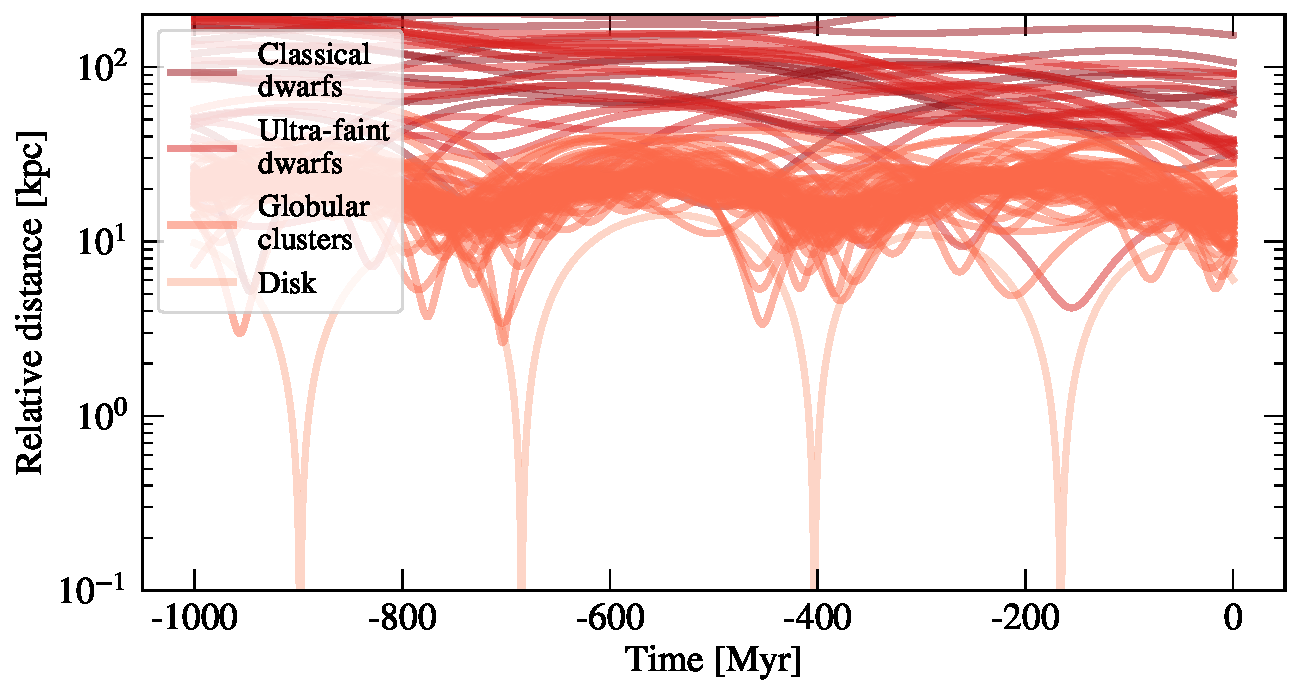
\includegraphics[width=\textwidth]{satellite_distances.pdf}
\end{center}
\caption{Data from \citet{simon2018} and \citet{gdr2_satellites}.}
\label{fig:known_encounters}
\end{figure}




\bibliographystyle{aasjournal}
\bibliography{spur}

\end{document}
